\documentclass[10pt]{article}

% Specify the margins and text size.
\setlength{\textwidth}{6.4in}
\setlength{\textheight}{9.5in}
\setlength{\oddsidemargin}{0pt}
\setlength{\evensidemargin}{0pt}
\setlength{\topmargin}{0pt}
\setlength{\hoffset}{.05in}
\setlength{\voffset}{-.8in}

\setlength{\parskip}{5pt}
\setlength{\parindent}{0pt}

% Load some fonts and symbol packages
\usepackage{latexsym}
\usepackage{pifont}       % contains 'star' symbol for counterinsurgency handbook title
\usepackage{yfonts} 
\usepackage{amsmath}
\usepackage{amsfonts}

\usepackage{graphicx}     % actually, this is loaded by pstricks
\usepackage[T1]{fontenc}
\usepackage{ifthen}
\usepackage{pstricks,pst-func,pst-text,pst-node,multido,pst-plot,calc,pst-3dplot}
%\usepackage[all]{xy}
%\usepackage{animate}

% The hyperref package inserts links into the pdf.
\definecolor{MyLinkColor}{rgb}{.1,.2,1}
\definecolor{MyCiteColor}{rgb}{.1,1,.2}
\definecolor{MyURLColor}{rgb}{.4,.4,.4}
\usepackage[backref=true,pagebackref=false,hyperindex,colorlinks=true,
  linkcolor=MyLinkColor,urlcolor=MyURLColor]{hyperref}


% The tweaklist package is something I found on the web.  It provides a simple interface
% for making changes to spacing used in the itemize and enumerate environments.  Comment
% this out if you don't care to use tweaklist.
\usepackage{tweaklist}
\renewcommand{\itemhook}{\setlength{\parskip}{2pt}\setlength{\parsep}%
{1pt}\setlength{\topsep}{0pt}\setlength{\itemsep}{0pt}}

\newcommand{\N}{\ensuremath\mathbb{N}}
\newcommand{\Q}{\ensuremath\mathbb{Q}}
\newcommand{\R}{\ensuremath\mathbb{R}}
\newcommand{\C}{\ensuremath\mathbb{C}}
\newcommand{\z}{\hphantom{0}}

\begin{document}
\pagestyle{empty}

\href{http://www.shepherd.edu}{
\includegraphics[height=1.75cm]{logo-high-res.eps}}
\vspace{-1.69cm}

{\small{\ }\hfill
\begin{tabular}{cl}
%\hspace{5in} 
& Math 314:  Statistics\\
%                & Warmup Exercises\\
                & %15 February 2012
\end{tabular}
}
\medskip

\begin{center}
\textbf{\large Regression Exercises with \texttt{R}}
\end{center}
\medskip

{\setlength{\baselineskip}{1.05\baselineskip}


1. Use \texttt{R} to calculate the example from pages 132--133.\\
   \texttt{> x <- c(1, 3, 4, 5, 7)}\\
   \texttt{> y <- c(5, 9, 7, 1, 13)}\\
   \texttt{> source("http://www.adjoint-functors.net/SDline.R")}\\
   \texttt{> SDline(x, y)}\\
   \texttt{\ \ \ \$meanX=4, \$meanY=7, \$slope=2, \$correlation=0.4}\\[3pt]
   \texttt{> linearModel <- lm(y$\sim$x)}\\
   \texttt{> summary(linearModel)}\\
   \texttt{Coefficients:}\\
   \texttt{\hphantom{Coefficients}Estmate Std.~Error t value Pr(>|t|)}\\
   \texttt{(Intercept)            \ \  3.800\ \ \ \ \ \ 4.733 
             \ \ 0.803 \ \ \   0.481}\\
   \texttt{x\hphantom{(coefficient}    0.800\ \ \ \ \ \ 1.058  
             \ \ 0.756 \ \ \   0.505}\\
   \texttt{Residual standard error:  4.733 on 3 degrees of freedom}\\
   \texttt{Multile R-squared:~0.16, Adjusted R-squared:~-0.12}\\
   \texttt{F-statistic:~0.5714 on 1 and 3 DF, p-value:~0.5046}
\bigskip

2. Use \texttt{R} to plot the example from pages 132--133.\\
   \texttt{> x <- c(1, 3, 4, 5, 7)}\\
   \texttt{> y <- c(5, 9, 7, 1, 13)}\\
   \texttt{> plot(x, y)}\\
   \texttt{> lines(x, 2*x - 1, type="l")}\\
   \texttt{> lines(x, 0.8*x + 3.8, type="l")}%\vspace{-10pt}
\rput(7,0.5){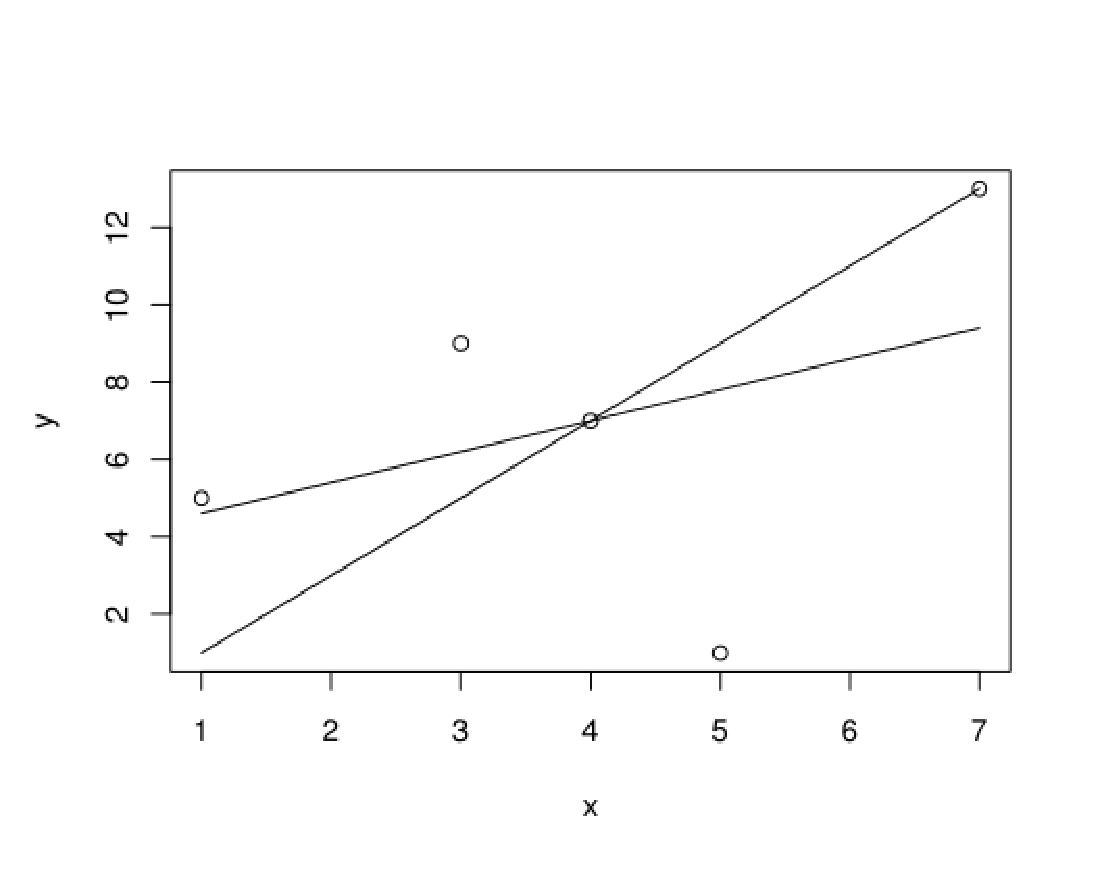
\includegraphics[height=1.8in,bb=-0 -0 515 350,clip]{Regress1.eps}}
\bigskip
\bigskip
\bigskip
\bigskip

3. Use the following to get the equation for the SD line of the
   \texttt{cars} data that is available in \texttt{R}.\\
 \texttt{> SDline(cars\$speed, cars\$dist)}\\
 \texttt{> plot(cars\$speed, cars\$dist)}\\
 Add the SD line to your plot.\\
 Use the following to get the regression line\\
 \texttt{> linearModel <- lm(cars\$dist$\sim$cars\$speed)}\\
 Add the regression line to your plot.\\
\vfill
\eject

\href{http://www.shepherd.edu}{
\includegraphics[height=1.75cm]{logo-high-res.eps}}
\vspace{-1.69cm}

{\small{\ }\hfill
\begin{tabular}{cl}
%\hspace{5in} 
& Math 314:  Statistics\\
%                & Warmup Exercises\\
                & %15 February 2012
\end{tabular}
}
\medskip

\begin{center}
\textbf{\large Regression Exercises}
\end{center}
\medskip

1. Consider the following data.
\begin{center}
\begin{tabular}{llll}
x: & average $\approx 100$, & $\mbox{SD}\approx 15$\\
y: & average $\approx 110$, & $\mbox{SD}\approx 30$,  & $r\approx 0.8$\\
\end{tabular}
\end{center}

\hspace{20pt} a) Predict the value of $y$ if $x=85$, $x=130$ and $x=\mbox{unknown}$.
\vspace{1.5in}

\hspace{20pt} b) Predict the value of $x$ if $y=95$, $y=140$ and $y=\mbox{unknown}$.
\vspace{1.5in}

2. Consider the following data.
\begin{center}
\begin{tabular}{llll}
x: & average $\approx 10$, & $\mbox{SD}\approx 2$\\
y: & average $\approx 12$, & $\mbox{SD}\approx 6$,  & $r\approx -0.2$\\
\end{tabular}
\end{center}

\hspace{20pt} a) Predict the value of $y$ if $x=6$, $x=16$ and $x=\mbox{unknown}$.
\vspace{1.5in}

\hspace{20pt} b) Predict the value of $x$ if $y=18$, $y=6$ and $y=\mbox{unknown}$.
\vspace{1.5in}

\vfill
\eject
{\ }

3. Consider the data from exercise 1. 

\hspace{20pt} a) Calculate the RMS error for regression.
\vspace{1.2in}

\hspace{20pt} b) Suppose $x=85$.  In what range does 68\% of the $y$-data fall?
\vspace{1.2in}

\hspace{20pt} c) Suppose $y=140$.  In what range does 95\% of the $x$-data fall?
\vspace{1.2in}


4. Consider the data from exercise 2. 

\hspace{20pt} a) Calculate the RMS error for regression.
\vspace{1.2in}

\hspace{20pt} b) Suppose $x=16$.  In what range does 68\% of the $y$-data fall?
\vspace{1.2in}

\hspace{20pt} c) Suppose $y=18$.  In what range does 95\% of the $x$-data fall?
\vspace{1.2in}

\end{document}
